% ===========================================================================
% HeteroDistill — Supplementary Material
% ===========================================================================
\documentclass[review,authoryear]{elsarticle}

\usepackage[T1]{fontenc}
\usepackage{lmodern}
\usepackage{textcomp}
\input{glyphtounicode}
\pdfgentounicode=1

\usepackage{graphicx}
\usepackage{amsmath}
\usepackage{amssymb}
\usepackage{booktabs}
\usepackage{multirow}
\usepackage{subcaption}
\usepackage{xcolor}
\usepackage{hyperref}
\usepackage{enumitem}

\journal{Automation in Construction}

\begin{document}

\begin{frontmatter}
\title{Supplementary Material for: HeteroDistill: Automated Crack and Spalling Segmentation for Concrete Dam Inspection via Heterogeneous Dual-Teacher Distillation}
\author[inst1]{Yanlin Chen\corref{cor1}}
\cortext[cor1]{Corresponding author.}
\address[inst1]{College of Graduate and Professional Studies, Trine University, Angola, IN 46703, USA}
\end{frontmatter}

\setcounter{section}{0}
\renewcommand{\thesection}{S\arabic{section}}
\renewcommand{\thetable}{S\arabic{table}}
\renewcommand{\thefigure}{S\arabic{figure}}
\renewcommand{\theequation}{S\arabic{equation}}

% ===========================================================================
\section{Agreement-Aware Knowledge Distillation}
\label{sec:supp_agreement}

When two teachers with different architectures and training recipes are combined, their predictions inevitably disagree at certain pixels---particularly at ambiguous crack--background boundaries and thin structures. At such pixels the ensemble soft label is unreliable, and forcing the student to match it may introduce noise. We note that high inter-teacher agreement does not guarantee correctness---both teachers may agree on an incorrect label---but empirically, agreement-weighted pixels yield more consistent supervision than disagreement regions.

We quantify per-pixel teacher agreement using the KL divergence between the two softened teacher distributions:
\begin{equation}
    d(i) = \text{KL}\!\left(\text{softmax}(\mathbf{z}_{T_1}^{(i)} / \tau) \,\|\, \text{softmax}(\mathbf{z}_{T_2}^{(i)} / \tau)\right)
    \label{eq:supp_teacher_disagree}
\end{equation}
where $i$ indexes spatial positions. An agreement map is derived as $a(i) = 1 - d(i) / \max_j d(j)$, ranging from 1 (full agreement) to 0 (maximum disagreement). The agreement-aware distillation loss modulates the per-pixel KD contribution:
\begin{equation}
    \mathcal{L}_{\text{KD}}^{\text{conf}} = \tau^2 \cdot \frac{1}{N} \sum_{i} a(i) \cdot \text{KL}\!\left(\tilde{\mathbf{p}}^{(i)} \,\|\, \text{softmax}(\mathbf{z}_s^{(i)} / \tau)\right)
    \label{eq:supp_conf_kd}
\end{equation}
The intent is that the student learns strongly from the ensemble where both teachers concur, but falls back on the ground-truth supervised loss at ambiguous pixels.

\textbf{Implicit sample-level effect.}
Because the loss is normalised by pixel count $N$ (not by $\sum_i a(i)$), an image with low overall agreement has lower total KD loss magnitude than one with high agreement. This means the formulation does \emph{not} operate purely at the pixel level: it also implicitly attenuates the KD loss for high-disagreement \emph{samples}. The sample-level reweighting ablation therefore does not fully isolate pixel-level from sample-level effects---both mechanisms are entangled in Eq.~\ref{eq:supp_conf_kd}.

\textbf{Technical limitations.}
The per-image max-normalisation $a(i) = 1 - d(i)/\max_j d(j)$ has several issues: (i)~division by zero when $\max_j d(j) = 0$ (handled by adding $\epsilon = 10^{-8}$); (ii)~the agreement map is scale-set by a single pixel (the most disagreeing one), making it sensitive to outliers; (iii)~KL divergence is asymmetric ($\text{KL}(T_1 \| T_2) \neq \text{KL}(T_2 \| T_1)$); (iv)~per-image normalisation makes the agreement values incomparable across samples.
Alternative designs (e.g., JS divergence, sum-normalisation, exponential decay, or fixed-threshold gating) may address these issues but are left to future work.

\begin{figure}[t]
    \centering
    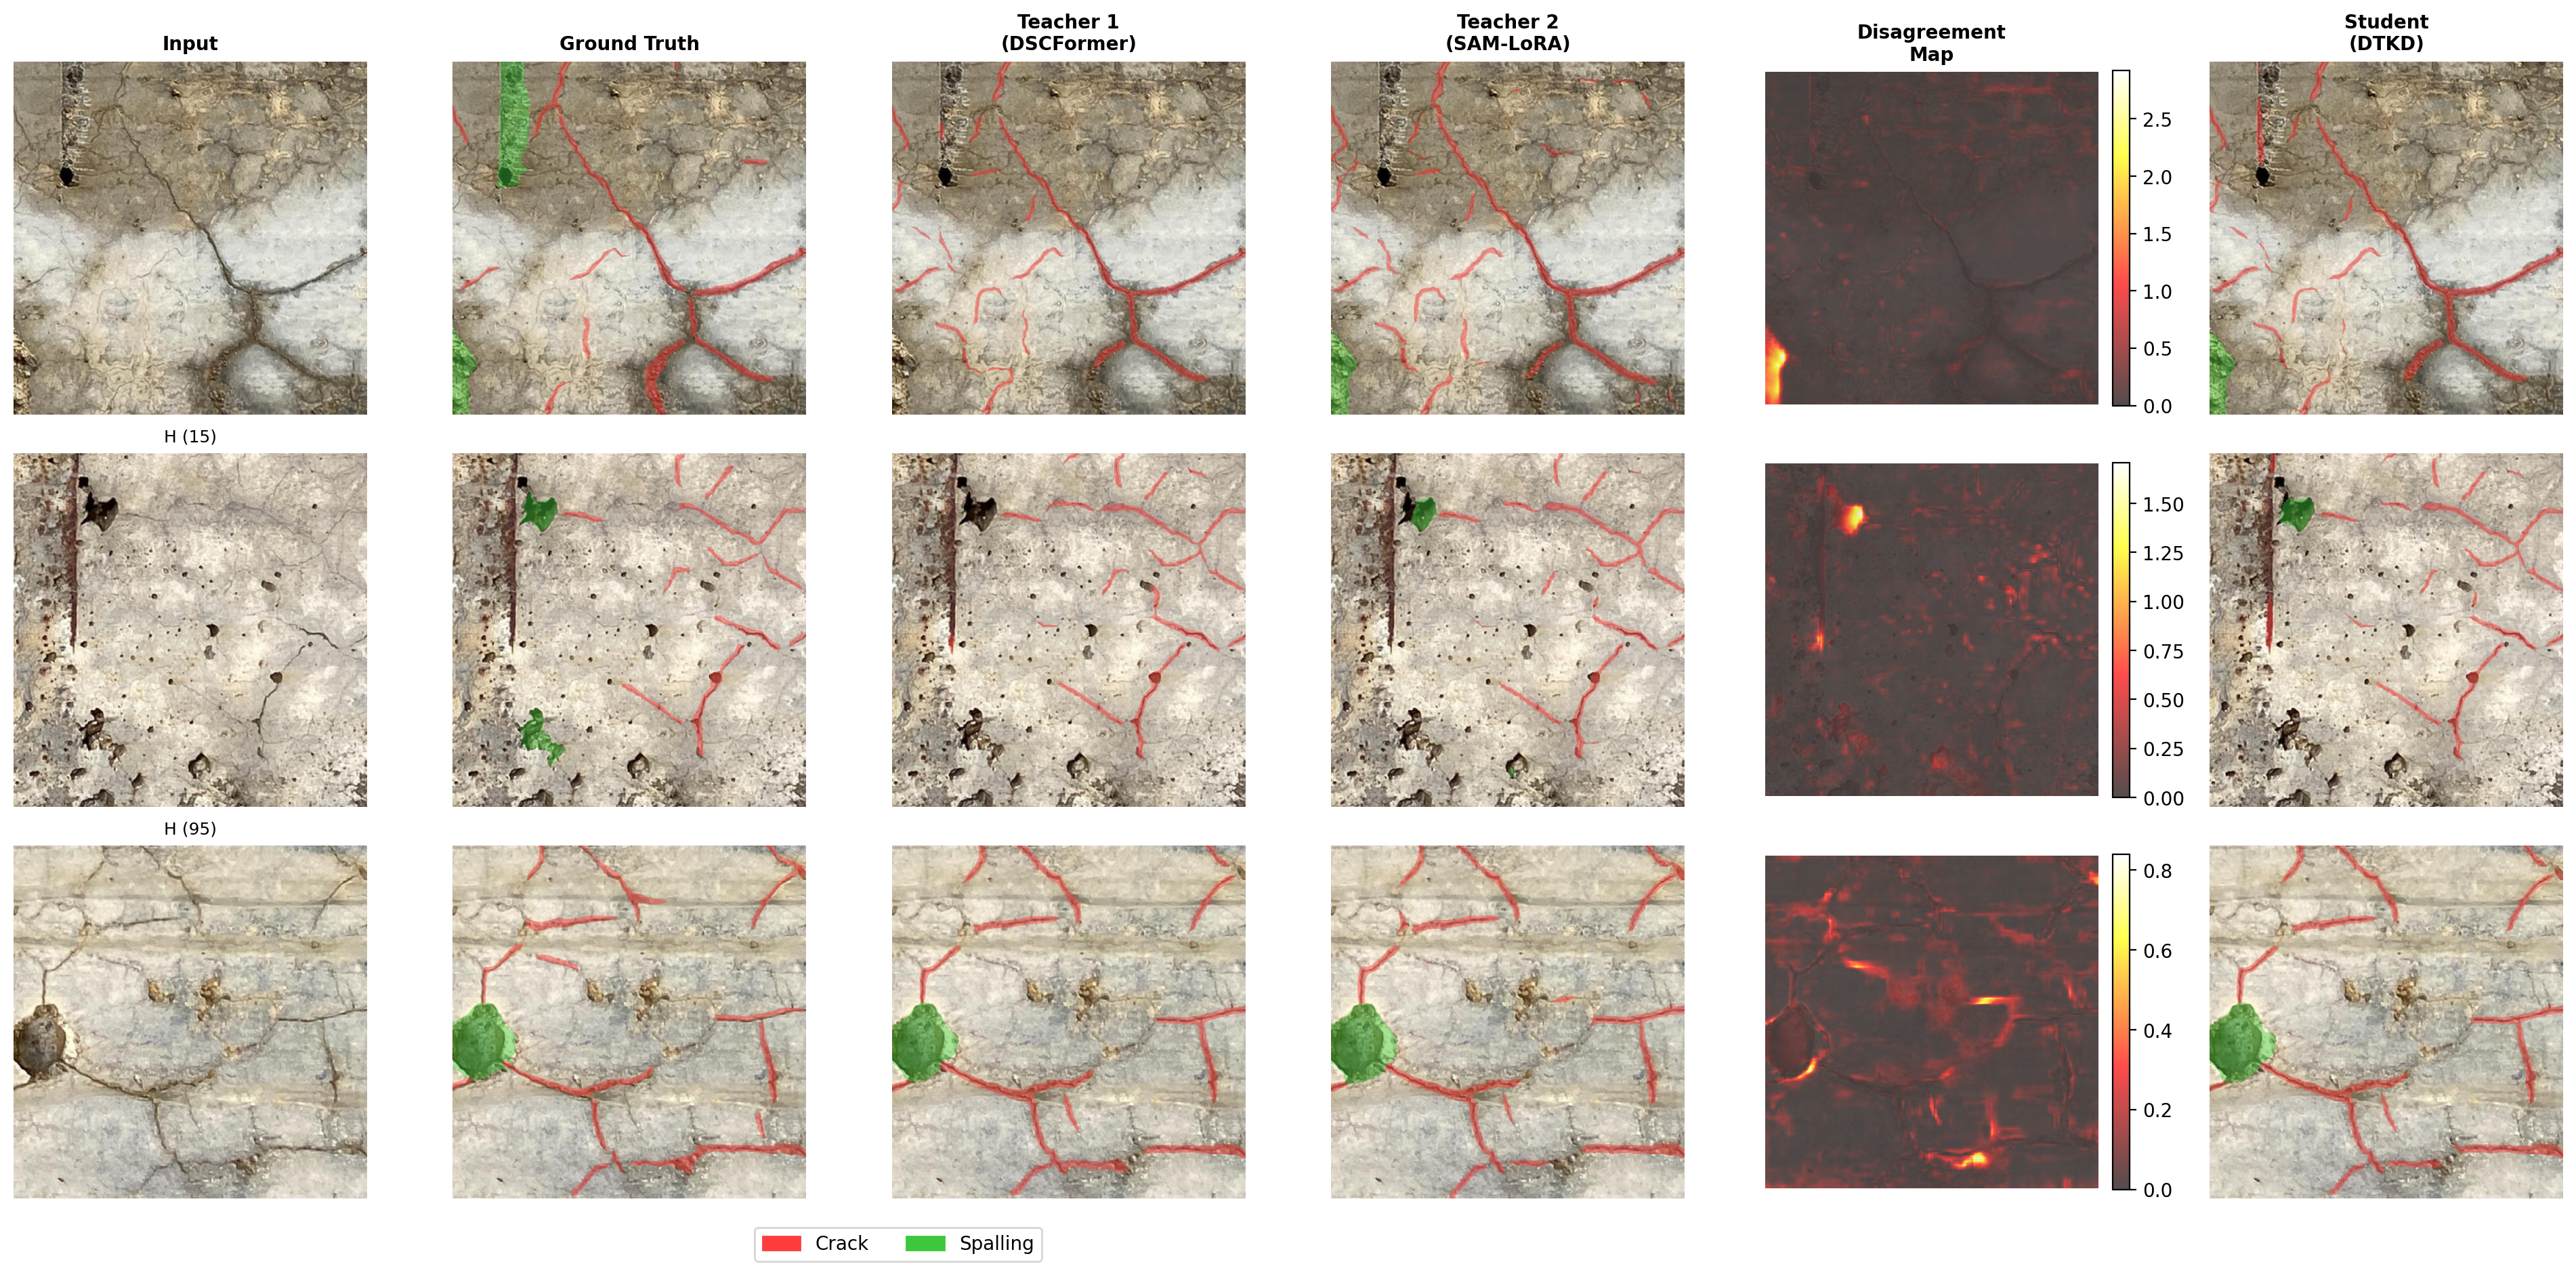
\includegraphics[width=\columnwidth]{figures/fig_agreement_map.png}
    \caption{Teacher disagreement visualisation on Hard-tier test samples containing both crack and spalling (randomly selected with seed 42). Columns: input, ground truth, Teacher~1 prediction, Teacher~2 prediction, pixel-level KL divergence heatmap (bright = high disagreement), student (DTKD) prediction. Disagreement tends to concentrate at crack boundaries and thin structures. Colourbar ranges are per-row (not unified). Red: crack, green: spalling.}
    \label{fig:supp_agreement}
\end{figure}

\paragraph{Agreement-aware KD ablation (row~g)}
Agreement-aware distillation improves boundary quality in a single run: BF1$_{\text{cr}}$ +0.8, clDice$_{\text{cr}}$ +0.6, mIoU$_{\text{fg}}$ +0.2 (within seed noise of 0.52). CompR$_{\text{cr}}$ decreases by $-$0.7. Multi-seed validation is needed.

An ablation using \emph{explicit} sample-level reweighting (without pixel-level modulation) degraded performance (mIoU$_{\text{fg}}$ 72.1, BF1$_{\text{fg}}$ 70.0), suggesting pixel-level modulation is the active mechanism. However, the agreement-aware KD loss contains implicit sample-level attenuation, so the two are not fully disentangled.
Teacher disagreement correlates with difficulty (+43\% KL divergence on Hard vs.\ Easy), but this does not translate into effective sample-level curriculum learning.

% ===========================================================================
\section{Per-Class Weighting Variant}
\label{sec:supp_perclass}

In addition to the equal-weight logit averaging (main paper Eq.~2), we explore a per-class probability-space variant:
\begin{equation}
    q_c = w_{1,c} \cdot p_{1,c} + w_{2,c} \cdot p_{2,c}, \qquad
    \tilde{p}_c = \frac{q_c}{\sum_{k} q_k}
    \label{eq:supp_perclass}
\end{equation}
where $p_{i,c} = \text{softmax}(\mathbf{z}_{T_i} / \tau)_c$ and $w_{1,c} + w_{2,c} = 1$ for each class $c$. We set $w_{2,\text{cr}} = 0.6$, $w_{2,\text{sp}} = 0.3$, $w_{2,\text{bg}} = 0.5$ (chosen manually, no systematic search).

\begin{table}[t]
\centering
\caption{Effect of teacher ensemble construction in DTKD. ``Equal'' (recommended default) uses logit-space averaging. ``Per-class'' uses probability-space per-class weighting. The near-identical performance confirms that DTKD's value derives from the dual-teacher ensemble rather than the specific mixing procedure. All values in \%.}
\label{tab:supp_kd_weights}
\begin{tabular}{lcccccc}
\toprule
Weighting & mIoU$_{\text{fg}}$ & IoU$_{\text{cr}}$ & IoU$_{\text{sp}}$ & BF1$_{\text{fg}}$ & clDice$_{\text{fg}}$ & CompR$_{\text{fg}}$ \\
\midrule
Equal (0.5/0.5) & 72.2 & 58.4 & 86.0 & \textbf{71.5} & 85.8 & \textbf{83.1} \\
Per-class & \textbf{72.3} & \textbf{58.5} & \textbf{86.2} & 70.6 & \textbf{86.4} & 83.0 \\
\bottomrule
\end{tabular}
\end{table}

% ===========================================================================
\section{Loss Function and Training Strategy Exploration}
\label{sec:supp_strategy}

\paragraph{Error analysis}
For crack pixels, precision is 68.8\% while recall is 79.7\%, yielding a false-positive to false-negative ratio of 1.78:1.
The majority of false positives occur at crack--background boundaries, where thin crack predictions leak into adjacent background pixels.

\paragraph{Strategy variants}
Table~\ref{tab:supp_strategy} summarises six training strategies applied on top of the DTKD pipeline, targeting crack precision improvement through loss modification or sampling adjustment.
Tversky loss \citep{salehi2017tversky} generalises Dice by introducing asymmetric FP/FN weights; WABL (Width-Aware Boundary Loss) applies an adaptive CE penalty at thin-crack boundary pixels; Boundary Dice restricts the Dice computation to a dilated boundary region around ground-truth contours.

\begin{table*}[t]
\centering
\caption{Training strategy exploration on the DamSegment test set. All variants build on HeteroDistill. ``Tversky $\alpha$'' controls FP penalty. WABL: Width-Aware Boundary Loss. Hard-tier FT: fine-tuning from the DTKD checkpoint with 70\% Hard-tier oversampling (30 additional epochs). All values in \%.}
\label{tab:supp_strategy}
\begin{tabular}{lcccccccc}
\toprule
Strategy & mIoU$_{\text{fg}}$ & IoU$_{\text{cr}}$ & IoU$_{\text{sp}}$ & BF1$_{\text{cr}}$ & BF1$_{\text{sp}}$ & BF1$_{\text{fg}}$ & clDice$_{\text{fg}}$ & CompR$_{\text{fg}}$ \\
\midrule
DTKD (CE+Dice) & 72.3 & 58.5 & 86.2 & 75.6 & 65.6 & 70.6 & 86.4 & 83.0 \\
\midrule
+ Tversky ($\alpha{=}0.6$) & 71.7 & 58.3 & 85.1 & 75.8 & 69.0 & \textbf{72.4} & 86.7 & 79.4 \\
+ Tversky ($\alpha{=}0.5$) & \textbf{72.1} & \textbf{58.9} & \textbf{85.4} & \textbf{76.4} & 65.7 & 71.0 & 86.5 & 81.1 \\
+ Boundary Dice & \textbf{72.1} & 58.8 & \textbf{85.4} & 75.7 & \textbf{69.2} & \textbf{72.4} & 86.4 & \textbf{83.2} \\
+ WABL & 71.6 & 58.4 & 84.8 & 75.9 & 64.0 & 70.0 & 84.9 & 79.5 \\
+ WABL + Tversky & 71.0 & 58.6 & 83.4 & 76.0 & 63.7 & 69.9 & 84.0 & 79.0 \\
\midrule
Hard-tier FT + WABL & 71.6 & 58.2 & 85.0 & 75.7 & 68.7 & 72.2 & \textbf{87.3} & 82.9 \\
\bottomrule
\end{tabular}
\end{table*}

A consistent crack--spalling tradeoff emerges: improving crack boundary precision degrades spalling metrics. No strategy surpasses the base DTKD model on mIoU$_{\text{fg}}$ (72.3), indicating that CE+Dice is already near-optimal for this dataset.

% ===========================================================================
\section{DTKD Hyperparameter Sensitivity}
\label{sec:supp_hyper}

\begin{table}[t]
\centering
\caption{DTKD hyperparameter star search (validation set, single run per setting with different random seeds). Differences within ${\sim}$1\% are within seed noise. All values in \%.}
\label{tab:supp_hyper}
\begin{tabular}{lcc}
\toprule
Setting & $(\alpha, \tau)$ & val mIoU$_{\text{fg}}$ \\
\midrule
$\tau{=}2$ & (0.5, 2) & 69.7 \\
$\tau{=}4$ (default) & (0.5, 4) & \textbf{71.1} \\
$\tau{=}6$ & (0.5, 6) & 71.4 \\
\midrule
$\alpha{=}0.7$ (more KD) & (0.7, 4) & 71.0 \\
$\alpha{=}0.5$ (default) & (0.5, 4) & \textbf{71.1} \\
$\alpha{=}0.3$ (less KD) & (0.3, 4) & 70.2 \\
\bottomrule
\end{tabular}
\end{table}

Excluding $\tau{=}2$ ($-$1.4\%, consistent with overly sharp teacher signals), all settings fall within 0.9\% of the default---well within seed noise (std $\approx$ 0.5). We retain $\tau{=}4$, $\alpha{=}0.5$ without claiming optimality.

% ===========================================================================
\section{Inference-Time Ensemble Analysis}
\label{sec:supp_ensemble}

To validate the premise underlying DTKD---that architecturally diverse models produce complementary error patterns---we perform inference-time logit ensembles of trained models without retraining (Table~\ref{tab:supp_ensemble}).

\begin{table}[t]
\centering
\caption{Inference-time ensemble analysis. Logit averaging of trained models (no retraining). ``G0'' = branch-augmented SegFormer (seed 42), ``SAM2'' = SAM-LoRA, ``G0-s$i$'' = G0 with different seed. TTA uses scales $\{0.75, 1.0, 1.25\}$ with horizontal flip. All values in \%.}
\label{tab:supp_ensemble}
\begin{tabular}{lcccccc}
\toprule
Ensemble & \#M & mIoU$_{\text{fg}}$ & IoU$_{\text{cr}}$ & BF1$_{\text{cr}}$ & clDice$_{\text{cr}}$ & CompR$_{\text{cr}}$ \\
\midrule
G0 (single) & 1 & 71.5 & 57.8 & 74.9 & 82.5 & 80.3 \\
G0 + G0-s2024 & 2 & 71.6 & 58.1 & 75.8 & 83.3 & 80.7 \\
G0 + SAM2 & 2 & 72.1 & 58.6 & 76.1 & 84.1 & 81.9 \\
G0 + SAM2 + G0-s2024 & 3 & \textbf{72.4} & \textbf{58.8} & \textbf{76.6} & 84.4 & 81.1 \\
\midrule
\multicolumn{7}{l}{\emph{With TTA:}} \\
G0 + TTA & 1 & 71.9 & 59.1 & 75.7 & 83.3 & 80.1 \\
G0 + G1 + SAM2 + G0-s123 + TTA & 4 & \textbf{72.5} & \textbf{59.8} & \textbf{77.4} & \textbf{84.9} & 80.4 \\
\bottomrule
\end{tabular}
\end{table}

Cross-architecture ensemble (G0~+~SAM2) yields 5$\times$ larger gains than same-architecture multi-seed ensemble (+0.56 vs.\ +0.10 mIoU$_{\text{fg}}$), supporting the DTKD premise that teacher diversity matters.

% ===========================================================================
\section{Engineering Quantities and Deployment Workflow}
\label{sec:supp_engineering}

\paragraph{From segmentation masks to engineering quantities}
Defect area is obtained by counting foreground pixels and converting via GSD. Crack length is estimated from the morphological skeleton, and connected components provide a defect-instance census.

\begin{table}[t]
\centering
\caption{Ground-truth engineering quantities for representative test patches (one per tier, median defect area among patches with both crack and spalling). Area and skeleton length assume GSD\,$=$\,1\,mm/pixel (illustrative). CC: connected components.}
\label{tab:supp_eng_quantities}
\setlength{\tabcolsep}{4pt}
\begin{tabular}{lrrrrr}
\toprule
Tier & Cr area (mm$^2$) & Sp area (mm$^2$) & Cr CC & Sp CC & Cr skel (mm) \\
\midrule
Easy   & 1{,}146  & 28{,}106 & 1  & 1 & 159 \\
Medium & 7{,}306  & 13{,}439 & 2  & 1 & 604 \\
Hard   & 30{,}278 & 2{,}780  & 50 & 1 & 4{,}514 \\
\bottomrule
\end{tabular}
\end{table}

\paragraph{Deployment workflow}
HeteroDistill is envisioned as the segmentation module in a multi-stage dam inspection pipeline:
(1)~UAV/camera capture;
(2)~tile into 512${\times}$512 patches;
(3)~HeteroDistill segmentation at 51 FPS (this paper);
(4)~post-processing for area, components, skeleton, continuity;
(5)~stitch into georeferenced defect map;
(6)~engineer review and prioritisation.
This paper addresses step~3 only.

% ===========================================================================
\section{Feature-Cluster Split Sanity Check}
\label{sec:supp_cluster}

To partially assess near-duplicate leakage, we constructed a feature-cluster split (ResNet-50 features, agglomerative clustering, 100 groups) after all design decisions were locked. All models were retrained.

\paragraph{Caveats}
The cluster split differs substantially from the original in size and composition: 631/369/500 (train/val/test) with imbalanced tiers (21/41/38\% Easy/Medium/Hard), vs.\ the original 1{,}200/150/150 with balanced tiers. Five of six models score \emph{higher} on the cluster split despite the smaller training set; the reason is unknown. The two test sets are therefore \emph{not directly comparable}.

\begin{table}[t]
\centering
\caption{Feature-cluster split sanity check. ``Orig.''$=$original split; ``Cluster''$=$feature-cluster split. The two test sets differ in size, tier composition, and difficulty, so absolute values are \emph{not directly comparable}. Models do not collapse under this split, but DTKD's ranking advantage is not preserved. All values in \%.}
\label{tab:supp_group_split}
\setlength{\tabcolsep}{4pt}
\begin{tabular}{lcccccc}
\toprule
\multirow{2}{*}{Model} & \multicolumn{2}{c}{mIoU$_{\text{fg}}$} & \multicolumn{2}{c}{BF1$_{\text{crack}}$} & \multicolumn{2}{c}{clDice$_{\text{crack}}$} \\
\cmidrule(lr){2-3}\cmidrule(lr){4-5}\cmidrule(lr){6-7}
 & Orig. & Clust. & Orig. & Clust. & Orig. & Clust. \\
\midrule
SegFormer-B2   & 70.4 & 73.0 & 73.7 & \textbf{78.3} & 81.9 & 85.0 \\
Mask2Former    & 67.9 & 70.2 & \textbf{76.0} & 75.0 & 82.2 & 81.5 \\
DSConv (row b) & 70.4 & \textbf{73.3} & 75.0 & 78.0 & 81.8 & 84.3 \\
DSConv+SRL (T1) & 70.6 & 73.1 & 74.7 & 78.2 & 82.5 & \textbf{85.7} \\
SAM-LoRA (T2)  & 68.1 & 65.3 & 73.1 & 72.9 & 81.3 & 80.2 \\
DTKD (ours)    & \textbf{72.3} & 72.7 & 75.6 & 76.4 & \textbf{83.3} & 84.0 \\
\bottomrule
\end{tabular}
\end{table}

This split addresses only \emph{visual} near-duplicates; patch coordinates were unavailable, so spatial leakage remains possible. This experiment is a partial sanity check, not a leakage proof.

% ===========================================================================
\section{Extended Metric Definitions}
\label{sec:supp_metrics}

\begin{itemize}[nosep]
    \item \textbf{CompP}: Component Precision---fraction of \emph{predicted} connected components for which $\geq$50\% of pixels overlap with GT pixels of the same class. CompP penalises spurious predicted components.
    \item \textbf{CompF1}: Harmonic mean of CompR and CompP, balancing recall of GT components with precision of predicted components.
    \item \textbf{PathCont}: Path Continuity---for each GT connected component, we extract its morphological skeleton and identify skeleton endpoints (pixels with exactly one 8-connected skeleton neighbour). A component is ``testable'' if its skeleton has $\geq$2 endpoints. PathCont is the fraction of testable GT components whose skeleton endpoints are mutually reachable through the predicted mask. PathCont captures whether the prediction preserves end-to-end connectivity of elongated structures.
\end{itemize}

% ===========================================================================
\section{Teacher Selection Ablation}
\label{sec:supp_teacher_selection}

Replacing Teacher~1 (branch+SRL) with the SRL-free branch-only variant degrades the student by $-$1.2 mIoU$_{\text{fg}}$ (71.1\% vs.\ 72.3\%), concentrated in spalling (IoU$_{\text{sp}}$ $-$2.4). This suggests that SRL-trained teachers produce more effective soft supervision despite their own component coverage regression (single comparison; multi-seed validation needed).

% ===========================================================================
\section{Statistical Significance Details}
\label{sec:supp_stats}

Paired Wilcoxon signed-rank tests (DSConv-only vs.\ HeteroDistill, 150 test images) show seven of ten per-class metrics reaching \emph{uncorrected} significance at $\alpha{=}0.05$: six favour DTKD---IoU$_{\text{cr}}$ ($p{=}0.008$), Dice$_{\text{cr}}$ ($p{=}0.007$), BF1$_{\text{cr}}$ ($p{=}0.046$), clDice$_{\text{cr}}$ ($p{<}0.001$), IoU$_{\text{sp}}$ ($p{=}0.016$), Dice$_{\text{sp}}$ ($p{=}0.016$)---while CompR$_{\text{cr}}$ decreases ($p{=}0.040$). After Holm--Bonferroni correction for 10 comparisons, only clDice$_{\text{cr}}$ ($p_{\text{adj}}{=}0.010$) survives; directional consistency is encouraging but per-class IoU gains are not confirmed after correction. Spalling sample sizes are small ($n{=}31$--40). Tier-stratified analysis shows the strongest effects on Hard images (IoU$_{\text{cr}}$ $p{=}0.003$, clDice$_{\text{cr}}$ $p{<}0.001$, uncorrected).

% ===========================================================================
\section{Cross-Dataset Evaluation Details}
\label{sec:supp_cross_dataset}

\textbf{Open-set rejection.} S2DS contains five defect classes absent from DamSegment (corrosion, efflorescence, vegetation, exposed reinforcement, control point), all mapped to background. The evaluation therefore conflates domain shift with open-set rejection.

\textbf{Caveats.}
The decomposition from branch-only (14.9\%) to branch+SRL (17.1\%) to HeteroDistill (18.7\%) is \emph{not} a clean ablation:
(i)~HeteroDistill simultaneously adds DTKD and removes student SRL;
(ii)~SegFormer-B2's near-zero transfer likely reflects class collapse;
(iii)~the branch modifies only the crack channel, yet the largest gains appear in spalling IoU;
(iv)~all results are single-seed and conflate domain shift with open-set rejection, and the $2{\times}$ downsampling may delete fine crack annotations.

\begin{figure}[t]
    \centering
    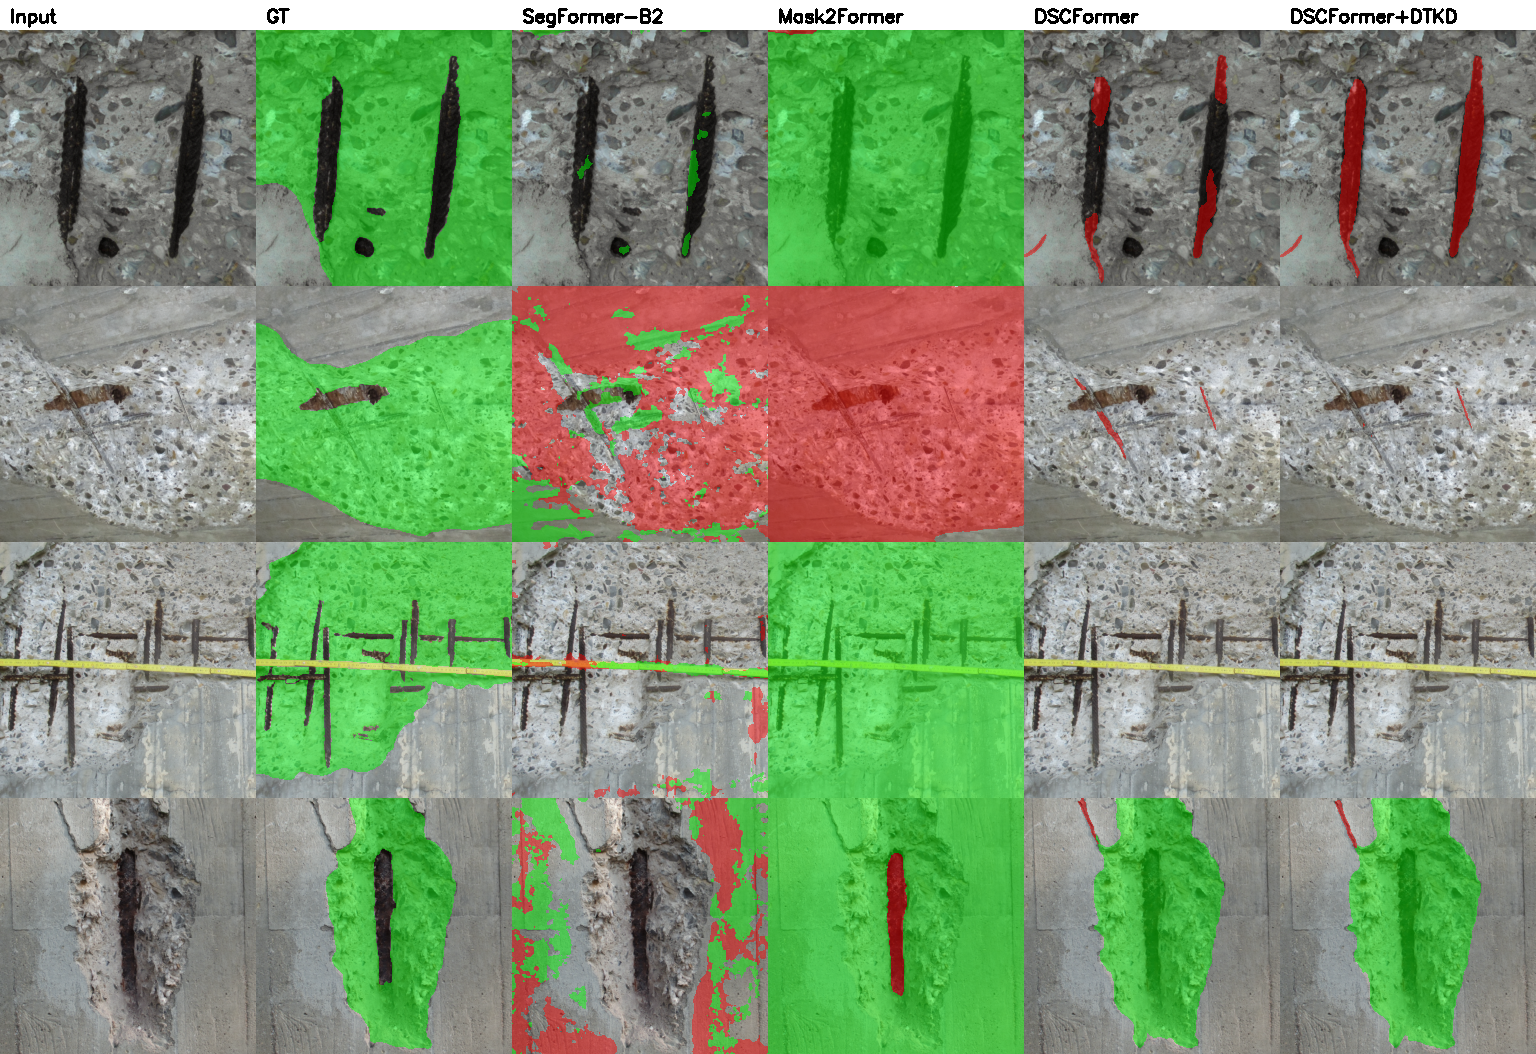
\includegraphics[width=\columnwidth]{figures/fig_cross_dataset.png}
    \caption{Cross-dataset qualitative results on S2DS (zero-shot). Left to right: input, ground truth, SegFormer-B2, Mask2Former, DSConv+SRL, HeteroDistill. Red: crack, green: spalling. Note visible over-prediction at region boundaries.}
    \label{fig:supp_cross_dataset}
\end{figure}

% ===========================================================================
\bibliographystyle{elsarticle-harv}

\begin{thebibliography}{9}

\bibitem[Salehi et~al.(2017)]{salehi2017tversky}
Salehi, S.S.M., Erdogmus, D., Gholipour, A., 2017.
\newblock Tversky loss function for image segmentation using 3D fully convolutional deep networks.
\newblock In: MLMI Workshop, MICCAI. Springer, LNCS~10541. pp.~379--387.

\end{thebibliography}

\end{document}
